\section{Subglacial Channel Formation From a Single Moulin (SHAKTI)}
\subsection{Goals} %{{{
\begin{itemize}
	\item Learn to set up a subglacial hydrology simulation using the SHAKTI model (Subglacial Hydrology and Kinetic, Transient Interactions, \cite{Sommers2018}),
	\item Run a test with steady input into a single moulin to see an efficient drainage pathway develop from the moulin to the outflow, and obtain the corresponding effective pressure, hydraulic head, and basal water flux distributions.
\end{itemize} 

Go to \verb@trunk/examples/shakti/@ to do this tutorial.
%}}}
\subsection{Introduction}
The \verb@runme.m@ file and \verb@moulin.par@ go through the steps and basic structure to set up and run a subglacial hydrology model with steady input into a single moulin at the center of a 1 km square, tilted slab of ice. These files can be altered to create simulations on different domains and geometries, with different meltwater inputs (distributed or into moulins, steady or time-varying). The \verb@runme.m@ script is set up as three distinct steps, saving the model at each stage:
\begin{enumerate}
	\item Mesh generation
	\item Parameterization
	\item Hydrology solution
\end{enumerate}

\subsection{Mesh Generation}
Run step 1 in \verb@runme.m@ to generate an unstructured mesh on a 1 km square with typical element edge length of 20 m. This mesh shown here has 4,032 elements and 2,096 vertices. To plot your mesh, use \verb@plotmodel(md,'data','mesh')@:
\begin{figure}[H]
	\begin{center}
		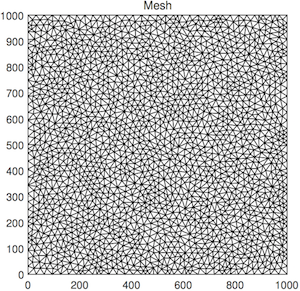
\includegraphics{/assets/img/using-issm/tutorials/shakti/moulin_mesh.png}
	\end{center}
\end{figure}


\subsection{Parameterization}
Run step 2 in \verb@runme.m@ to define the model parameters. First we call on standard parameters defined in the \verb@moulin.par@ file (bed and ice geometry, sliding velocity, material properties, etc.). Then we define hydrology-specific parameters for the SHAKTI model (initial hydraulic head, Reynolds number, subglacial gap height, boundary conditions, etc.).

The model domain is set up as a 500 m thick slab of ice, with bed and surface slope of 0.02. We begin by assuming the hydraulic head is such that the water pressure is equal to 50\% of the ice overburden pressure, Re=1,000 everywhere, and the initial gap height is 0.01 m. The outflow boundary (x=0 m) is set to atmospheric pressure ($h=z_b$) with a "Type 1" (Dirichlet) condition. We set the distributed input from the englacial system to the subglacial system as zero (for this example, we will define the moulin input in the next step).

To look at the bed topography, ice surface, initial head, and initial gap height, you can plot them in MATLAB:

\begin{verbatim}plotmodel(md,...
'data',md.geometry.base,'title','Bed Elevation [m]',...
'data',md.geometry.surface,'title','Surface Elevation [m]',...
'data',md.hydrology.head,'title','Initial Head [m]',...
'data',md.hydrology.gap_height,'title','Initial Gap Height [m]')\end{verbatim}

\begin{figure}[H]
	\begin{center}
		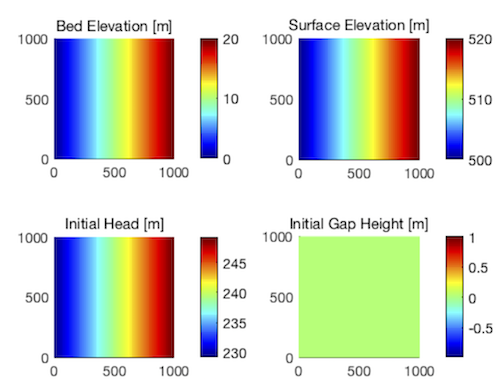
\includegraphics{/assets/img/using-issm/tutorials/shakti/moulin_initial.png}
	\end{center}
\end{figure}

\subsection{Hydrology solution}
In step 3, we specify which machine we want to run the model on, including number of processors to be used, define the model time step, final time, and prescribe the moulin inputs. In this example, we put a steady moulin input of 4 m$^3$ s$^{-1}$ at the center of the domain (x=500 m, y=500 m). We also impose a no-flux "Type 2" (Neumann) boundary condition at all boundaries (except the outflow, where we have our Dirichlet condition defined already in step 2).

Now that the set up is complete, we can run the model:
\begin{verbatim}md=solve(md,'Transient');\end{verbatim}

The final steady configurations for effective pressure, hydraulic head, basal water flux, and gap height can be visualized by plotting:
\begin{verbatim}plotmodel(md,'data',md.results.TransientSolution(end).EffectivePressure,'title','Effective Pressure [Pa]',...
'data',md.results.TransientSolution(end).HydrologyHead,'title','Head [m]',...
'data',md.results.TransientSolution(end).HydrologyBasalFlux,'title','Basal Water Flux [m^2 s^{-1}]',...
'data',md.results.TransientSolution(end).HydrologyGapHeight,'title','Gap Height [m]')\end{verbatim}

\begin{figure}[H]
	\begin{center}
		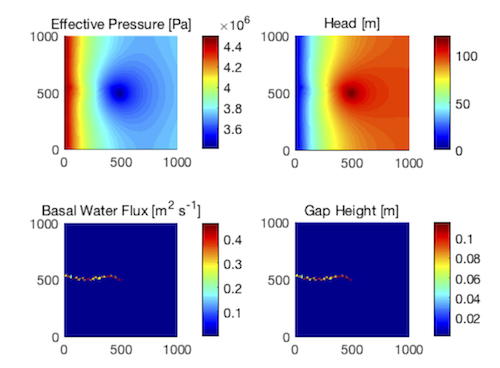
\includegraphics{/assets/img/using-issm/tutorials/shakti/moulin_final.png}
	\end{center}
\end{figure}

You can see that a distinct pathway has formed from the moulin at the center to the outflow at the left. Hydraulic head (related to water pressure) is highest directly around the moulin, and the head is lower in the channel than in the areas above and below it in the y-direction. 

To watch the evolution through time in an animation, use the command: 
\begin{verbatim}plotmodel(md,'data','transient_movie')\end{verbatim}

You will be prompted to select which parameter to animate, and can watch an efficient subglacial channel emerge from the moulin to the outflow!
